\chapter{Revisão da Literatura}
\label{cap:02}
Graças ao avanço da tecnologia, o uso da energia elétrica se tornou extremamente vital, causando o aumento do uso de meios de geração por combustíveis fósseis, o qual gerou grande emissão de gás carbônico. De acordo com \citeauthorandyear{caldeira2003climate}, considerando um cenário para estabilização do clima e onde a sensibilidade climática se encontra no máximo apontado pelo IPCC, \textit{Intergovernmental Panel on Climate Change}, e assumindo o IPCC IaaS92a, ao final do século XXI a maior parte da geração de energia deverá ser estritamente de fontes não emissoras de $CO_{2}$.

\FloatBarrier
\begin{figure}[htbp]
	\centering
	%scale redimensiona a figura.
	%1.5 = 150% do tamanho original
	%1 = 100% do tamanho original
	%0.20 = 20% do tamanho original
	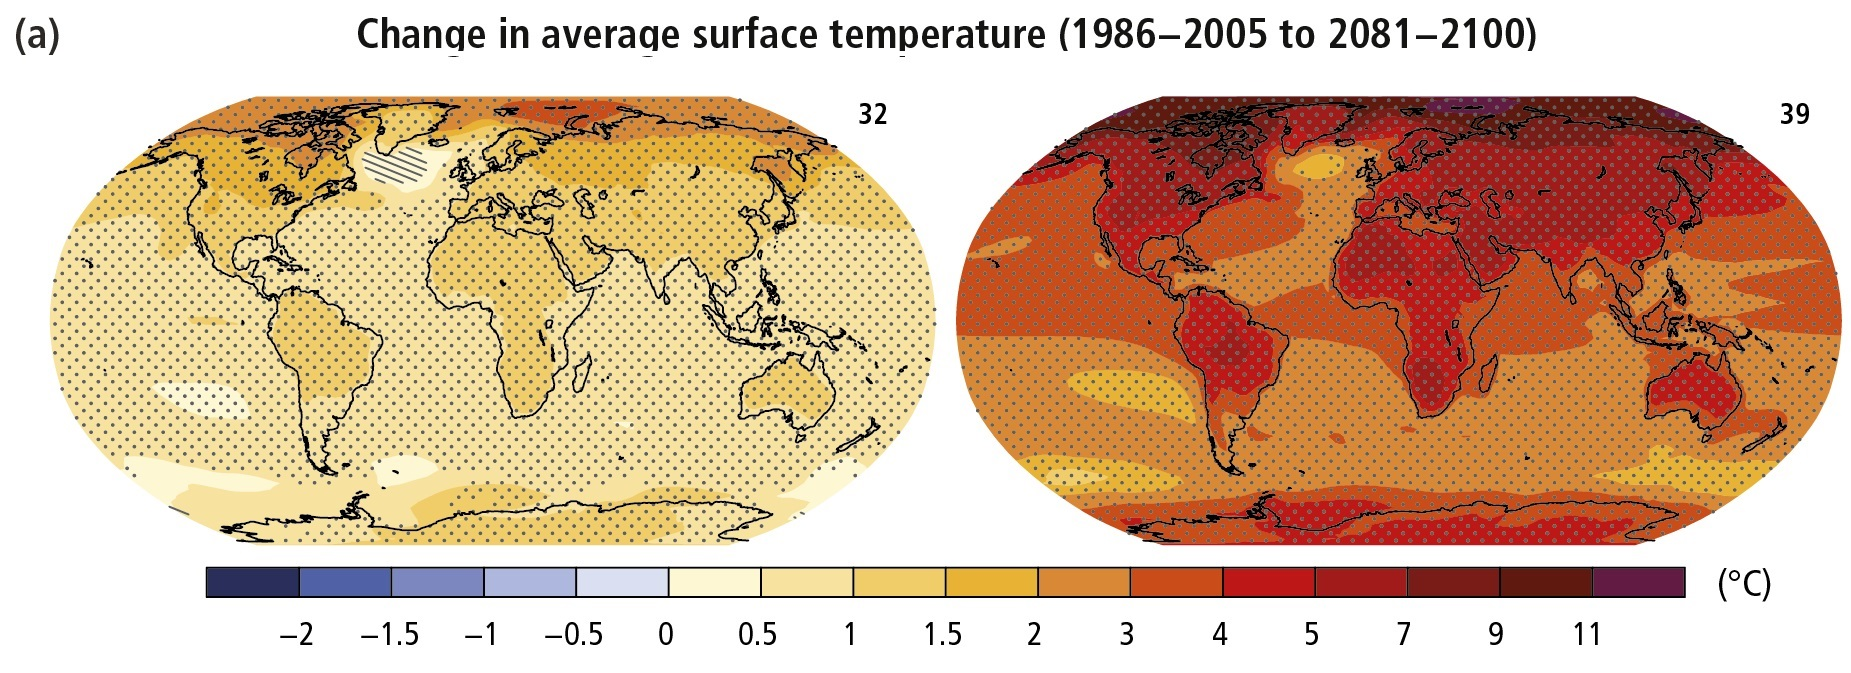
\includegraphics[scale=1.]{imagens/Temp_IPCC}
	\caption{Variação na temperatura geral da superfície da Terra durante os anos de 1986-2005 para 2081-2100. Fonte: IPCC. }
	
	\label{fig:TempE}
\end{figure}
\FloatBarrier


Como apontado por \citeauthorandyear{weitemeyer2015integration}, o uso de energias renováveis na Europa tem aumentado, considerando as preocupações em relação as alterações climáticas. Como citado pelo autor, devido à facilidade imposta pelo ambiente, considerando um objetivo onde o uso da geração será prioritariamente por fontes renováveis, tem-se o uso da energia solar e eólica como pontos chaves para se alcançar esse objetivo. Como simulado e mostrado na figura~\ref{fig:Wind_sol}, o uso de energias renováveis se mostra promissor na simulação considerando a Alemanha como objeto de estudo, tendo apenas a geração estrita por meio de energia solar, distante do cenário de integração perfeita, onde $\alpha$=0 representa uma geração estritamente solar, e $\alpha$=1 representa uma geração estritamente eólica.

\FloatBarrier
\begin{figure}[htbp]
	\centering
	%scale redimensiona a figura.
	%1.5 = 150% do tamanho original
	%1 = 100% do tamanho original
	%0.20 = 20% do tamanho original
	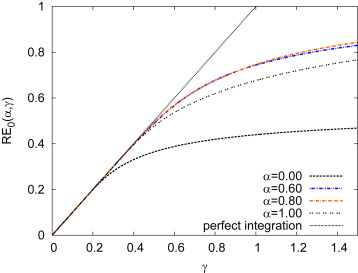
\includegraphics[scale=1.5]{imagens/wind_solar}
	\caption{Simulação do uso de energias renováveis na Alemanha, utilizando-se diferentes ponderações na divisão entre fontes de geração solar e eólica. Fonte:  \citeauthorandyear{weitemeyer2015integration} }
	
	\label{fig:Wind_sol}
\end{figure}
\FloatBarrier

Tendo em vista o problema causado por energias provenientes de fontes fósseis, o Brasil se concentrou na geração de energia elétrica de fontes renováveis principalmente hidráulicas, atingindo um índice de mais de 74\% de sua produção de acordo com \citeauthorandyear{wanderley2013perspectivas} e conforme visto na figura~\ref{fig:FonteEnergia}.

Devido a oscilações anuais dos índices de chuva, o racionamento de energia causado pelas épocas de estiagem, excitou a busca por novas fontes energéticas alternativas; tendo em vista que o Brasil é um país de clima predominantemente tropical, houve um crescente  desenvolvimento de pesquisas para a produção de energia solar fotovoltaica. 

\FloatBarrier
\begin{figure}[htbp]
	\centering
	%scale redimensiona a figura.
	%1.5 = 150% do tamanho original
	%1 = 100% do tamanho original
	%0.20 = 20% do tamanho original
	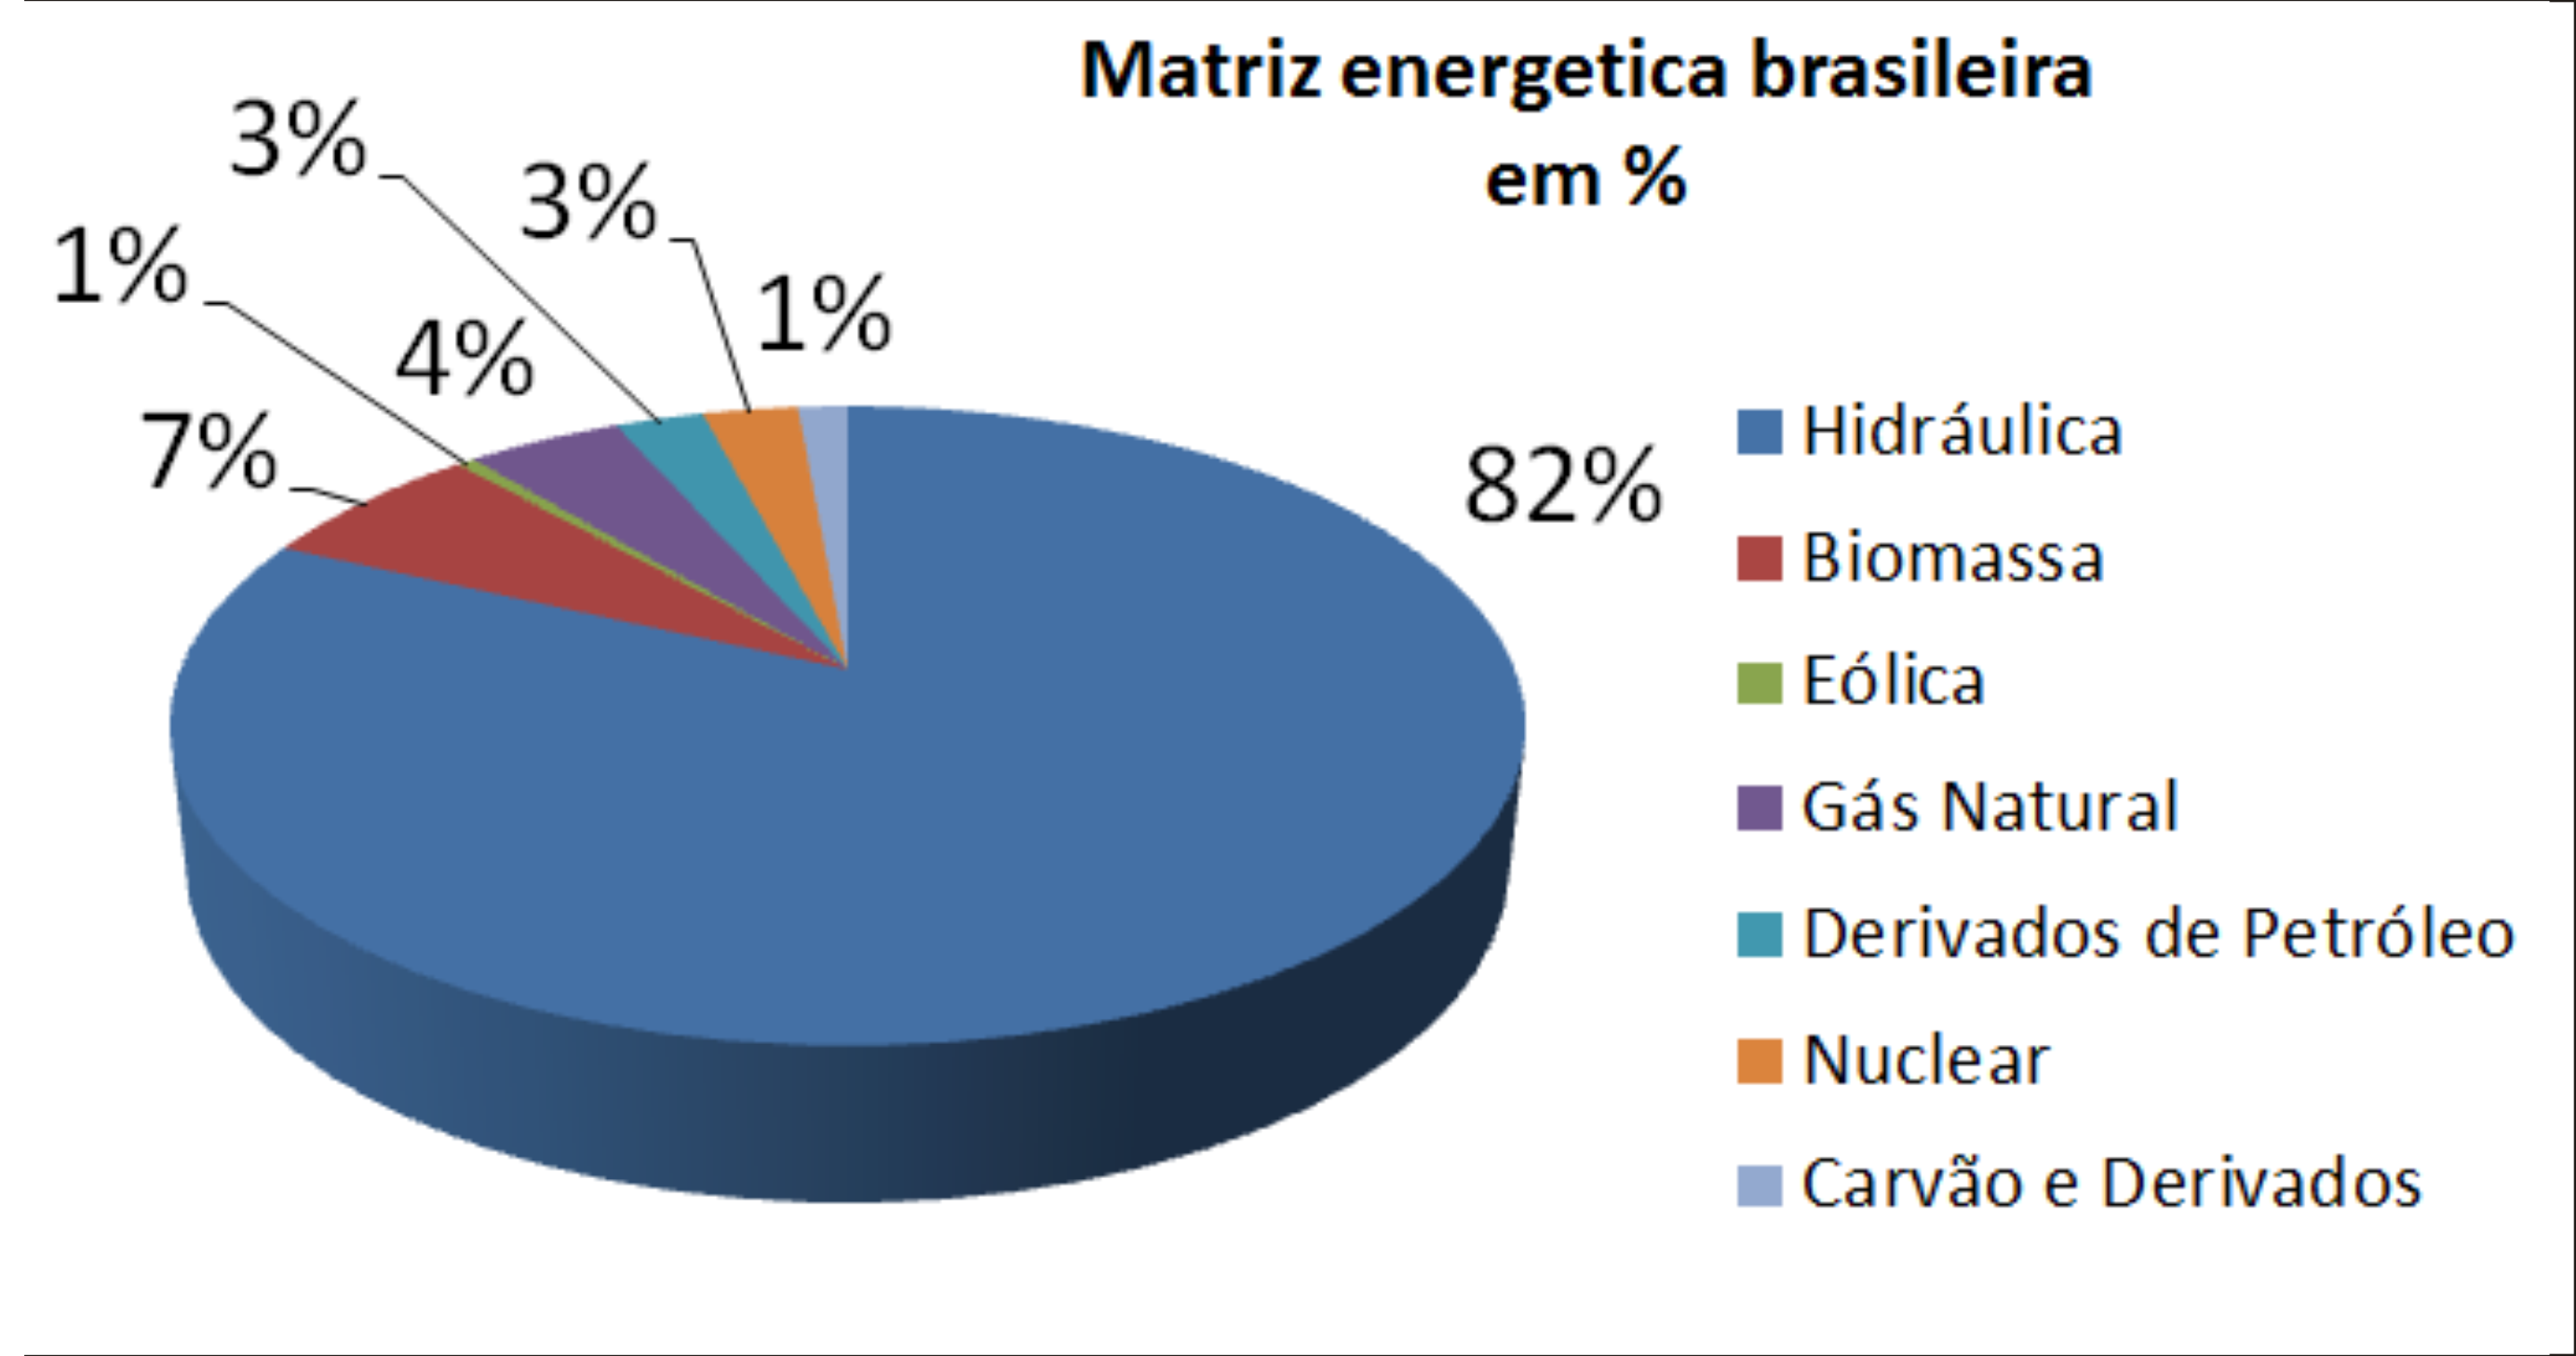
\includegraphics[scale=1]{imagens/FontesEnergia}
	\caption{Distribuição da matriz energética brasileira. Fonte:  \citeauthorandyear{wanderley2013perspectivas}. }
	
	\label{fig:FonteEnergia}
\end{figure}
\FloatBarrier

O grande impasse para produção de usinas solares é o alto valor de produção tendo em vista o rendimento dos painéis fotovoltaicos comparado  com as fontes de energias tradicionais. De acordo com \citeauthorandyear{ribeiro2017proposiccao}, para construir uma usina solar fotovoltaica com capacidade de produção de aproximadamente $4.000MWh$ ao ano, seria necessário um investimento de aproximadamente $R\$ 22.000.000,00$ ou seja, $7,30 R\$/Wp$; no artigo citado, foram taxados preços dos painéis, inversores, imposto de importação e taxas de produção. A solução para viabilizar a produção deste tipo de energia, seria o aumento de sua eficiência energética. Para alcançar este objetivo, foram efetuados diversos estudos, pesquisas e implementações de circuitos eletrônicos e projetos mecânicos.
 
Há trabalhos de pesquisa que visam obter o melhor aproveitamento da radiação solar criando sistemas mecânicos, \citeauthorandyear{WILLOUGHBY2018171},  enquanto alguns fazem comparações entre painéis com células obstruídas através de sombreamento \citeauthorandyear{BRESSAN20161181}, outros fazem a aplicação de diferentes aparatos para se obter energia perdida devido à difusão dos raios solares Lee et al. (2016), há trabalhos que propõem mensurar a perda de energia devido a poluição do ar em determinadas regiões \citeauthorandyear{li2017reduction}. Foram apresentados projetos que objetivam a melhora da potência entregue pelos painéis através no melhoramento da curva IxV (Corrente por tensão), foram apresentados projetos mostrando modos de melhoria desta curva, entre eles o algoritmo MPPT (Maximum Power Point Traking)\citeauthorandyear{WILLOUGHBY2018171}.  

\FloatBarrier
\begin{figure}[htbp]
	\centering
	%scale redimensiona a figura.
	%1.5 = 150% do tamanho original
	%1 = 100% do tamanho original
	%0.20 = 20% do tamanho original
	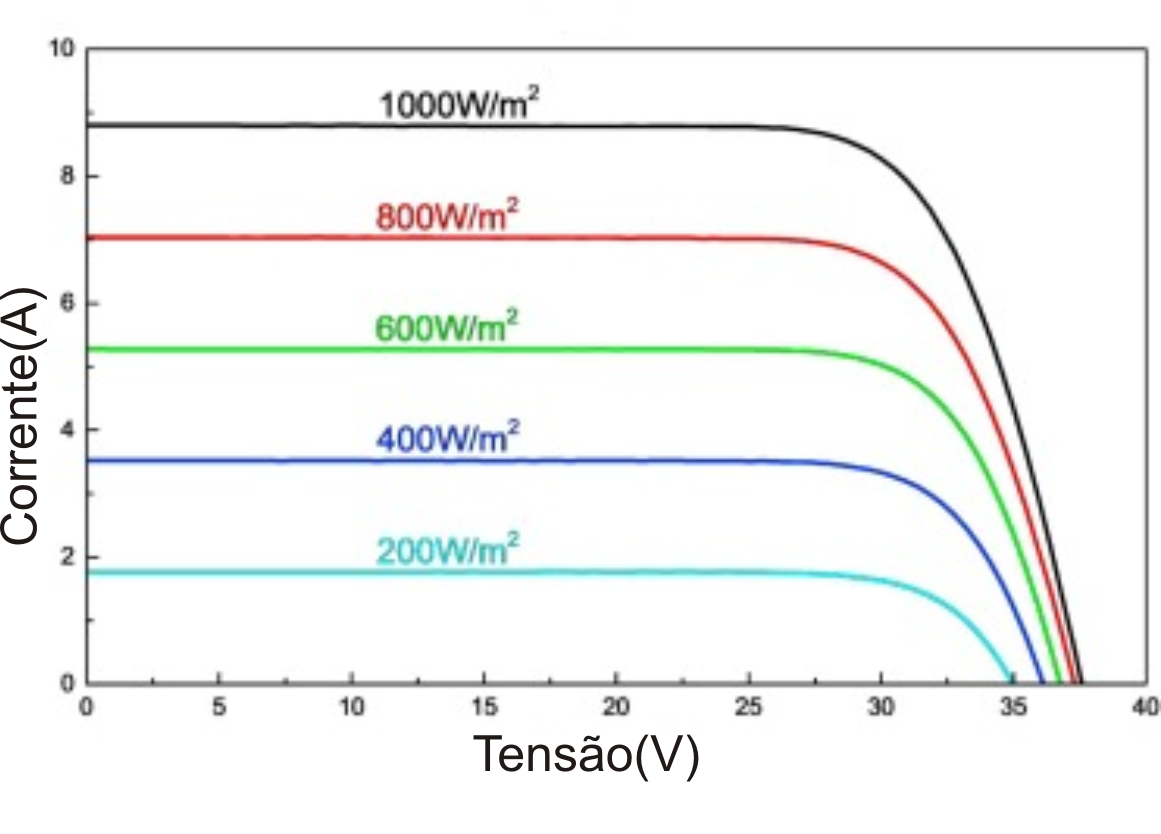
\includegraphics[scale=1.3]{imagens/IV_Gao}
	\caption{Curva IxV Característica de um painel fotovoltaico. Fonte:  \cite{GAO201852}.  }
	
	\label{fig:IVGao}
\end{figure}
\FloatBarrier

Para se obter um maior rendimento dos painéis fotovoltaicos, \citeauthorandyear{WILLOUGHBY2018171} apresentaram um projeto de um seguidor solar tendo por base um microcontrolador e motores de passo. A ideia proposta é a de que, durante o transcorrer do dia, o painel solar se modificaria sua inclinação de modo a estar sempre perpendicular a incidência dos raios solares, tendo assim uma potência de geração superior aos modelos convencionais com bases fixas.

Tomando uma abordagem diferente, porém com o mesmo intuito, Lee et al. (2016) publicaram \textit{Concentrator photovoltaic module architectures with capabilities for capture and conversion of full global solar radiation}. No artigo citado, foi apresentada a ideia de um concentrador de raios solares fazendo uso das células fotovoltaicas do tipo 3J (esférica) e 4J (plana). 

Foram propostas duas tecnologias de funcionamentos similares:

\begin{itemize}
	\item O primeiro concentrador é uma placa translúcida composto por bolhas que é colocada na parte de cima do painel com um distanciamento de 10 centímetros, essas bolhas tem como função captar os raios solares difusos e concentrar sobre células fotovoltaicas do tipo 3J;
	\item O segundo concentrador tem o mesmo princípio de funcionamento, uma placa translúcida com bolhas de estrutura diferente da apresentada anteriormente é colocada na parte superior do painel com um distanciamento de aproximadamente 10 centímetros, mas ao invés de concentrar os raios solares em uma única célula 3J, a bolha capta a irradiância solar e distribui de maneira uniforme sobre uma célula do tipo 4J.
\end{itemize}

Os dois métodos exibem resultados de até 8\% mais eficiência energética em comparação aos painéis fotovoltaicos convencionais, isso dado ao aumento da concentração e direcionamento dos raios solares difusos sobre as células fotovoltaicas.

Foi colocado por\cite{li2017reduction}, um ponto negativo e preocupante a respeito da produção de energia fotovoltaica no território da China. Segundo o artigo publicado: \textit{Reduction of solar photovoltaic resources due to air pollution in China}, A China tem por pretensão a produção de 400 $GW$ de energia elétrica proveniente de painéis fotovoltaicos até 2023. Porém, o estudo realizado revela que atualmente a poluição aérea causada por aerossóis, diminui de forma significativa a produção de energia fotovoltaica, em destaque na região do centro, leste e nordeste no país, locais de maior concentração de indústrias, índice de poluição e necessidade de energia elétrica. Índices mostram uma perda de 35\% da energia produzida e 1,5 $kWh/m^2$ da irradiância solar em todo território descrito, as nuvens causam grande influência sobre a irradiância solar que atinge o solo daquela região, porém com o agravante, as perdas aumentaram significativamente.

Assim como descrito anteriormente, painéis fotovoltaicos possuem diversas características favoráveis à geração de energia por meios sustentáveis e limpos. Entretanto, como aponta \citeauthorandyear{BRESSAN20161181}, arranjos fotovoltaicos estão extremamente sujeitos a meios externos que podem afetar sua geração, como sujeira, ou sombreamento, fatores os quais causam um rápido aquecimento das células fotovoltaicas. Existem maneiras de amenizar esse efeitos, como o uso de diodos \textit{bypass}, entretanto o uso dessas técnicas não anulam esse efeitos por completo. Como mostrado na Figura~\ref{fig:Temp}, é possível observar a variação da temperatura, alterando consequentemente o funcionamento do painel fotovoltaico.

\FloatBarrier
\begin{figure}[htbp]
	\centering
	%scale redimensiona a figura.
	%1.5 = 150% do tamanho original
	%1 = 100% do tamanho original
	%0.20 = 20% do tamanho original
	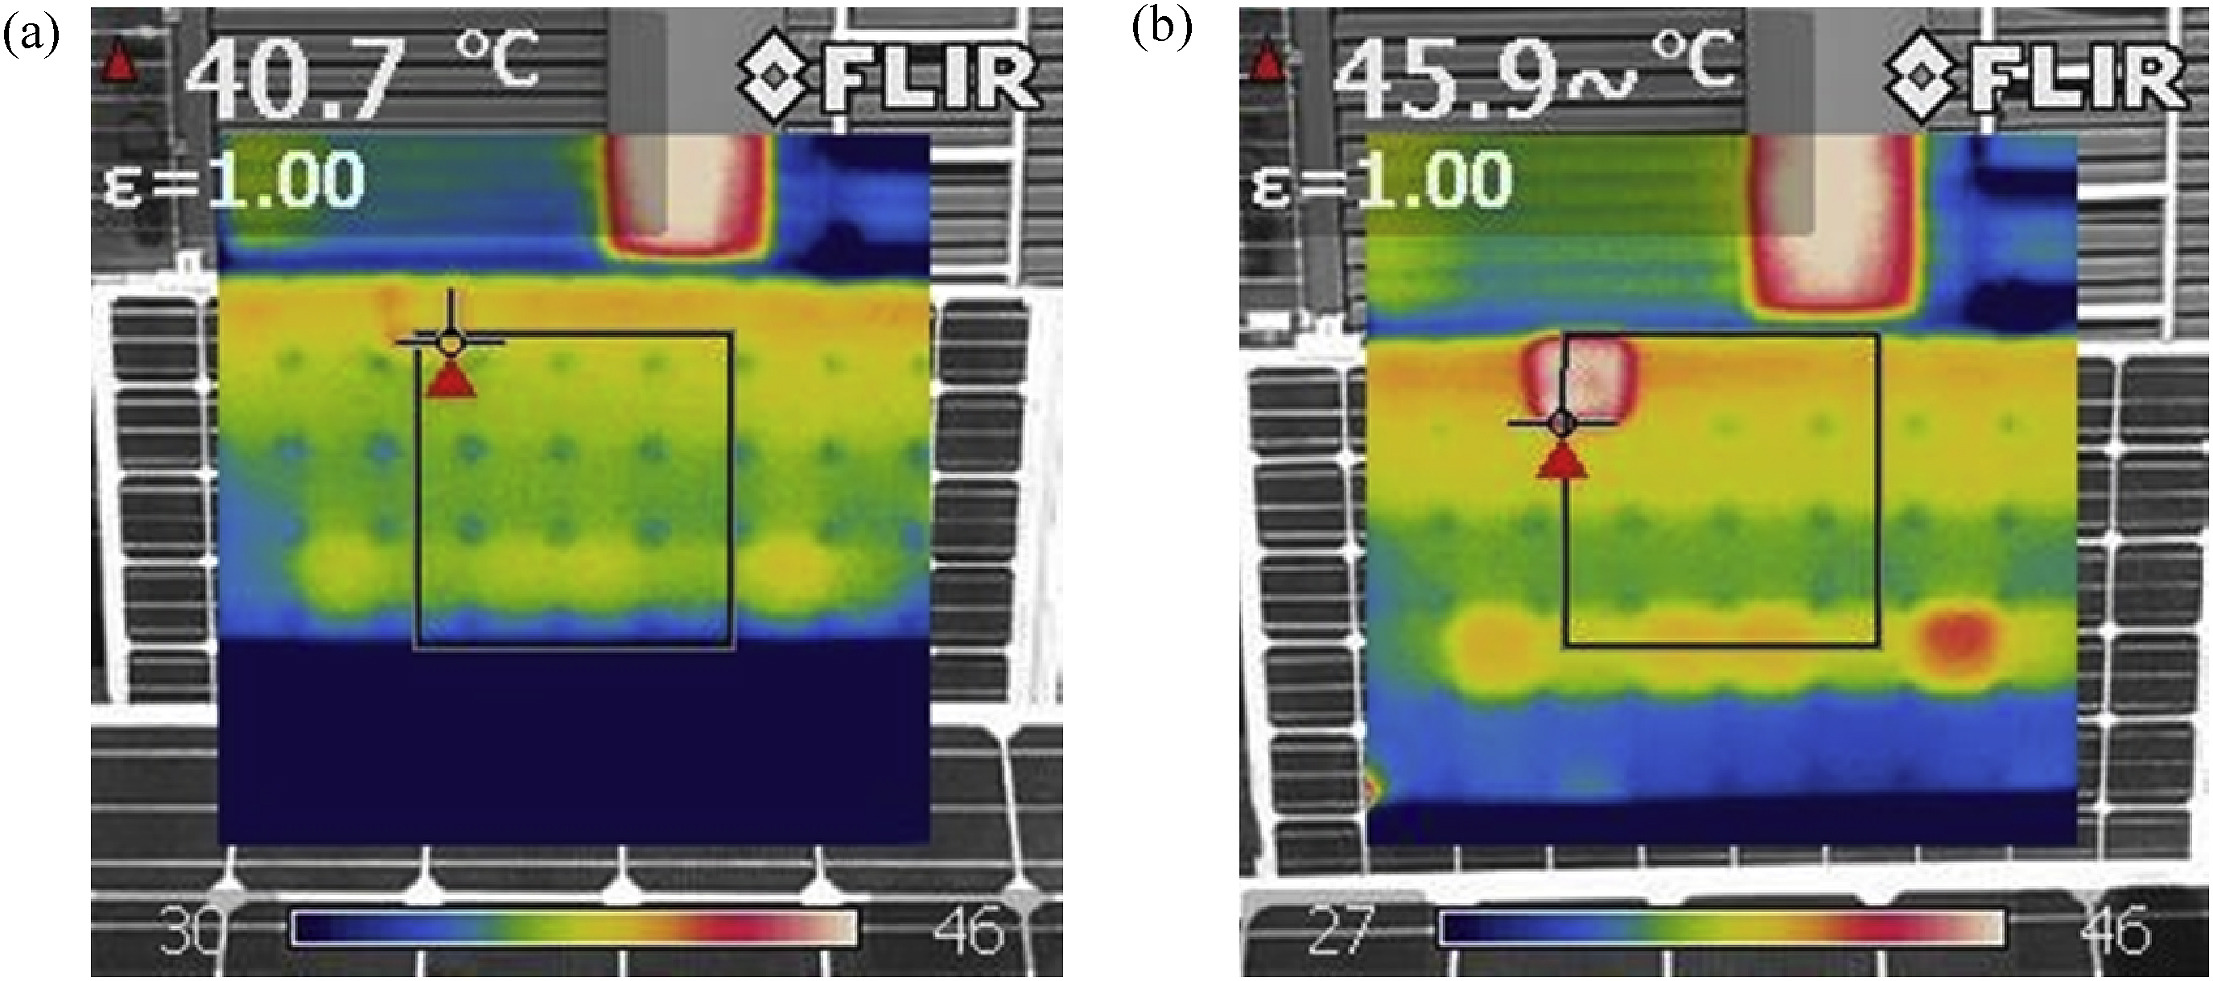
\includegraphics[scale=1.3]{imagens/Temp_BRESSAN}
	\caption{Variação na temperatura de células fotovoltaicas em um arranjo em curto-circuito. Fonte:  \citeauthorandyear{BRESSAN20161181} }
	
	\label{fig:Temp}
\end{figure}
\FloatBarrier

Como apontado anteriormente , há grande importância e interesse no uso da curva I-V de sistemas fotovoltaicos, para gerenciamento, funcionamento, e verificação de erros, assim como descreve \citeauthorandyear{SCHILL2015259} no \textit{Fraunhofer Institute for Solar Energy Systems ISE}, faz-se o uso da curva I-V para verificação da performance dos arranjos fotovoltaicos durantes teste em ambientes abertos para verificação da durabilidade de materiais para o uso em sistemas fotovoltaicos. De acordo com os autores, é verificado e monitorado a curva a cada 10 minutos. O uso da curva I-V permitiu a conclusão em teste onde os painéis foram sujos, durante o teste foi verificada uma diminuição de até 20\% dos valores iniciais de eficiência, sendo possível observar a diferença entre as curvas de placas limpas e placas sobre grande influência de poeira como visto na Figura~\ref{fig:CurvaIVNeve}.

\FloatBarrier
\begin{figure}[!htbp]
	\centering
	%scale redimensiona a figura.
	%1.5 = 150% do tamanho original
	%1 = 100% do tamanho original
	%0.20 = 20% do tamanho original
	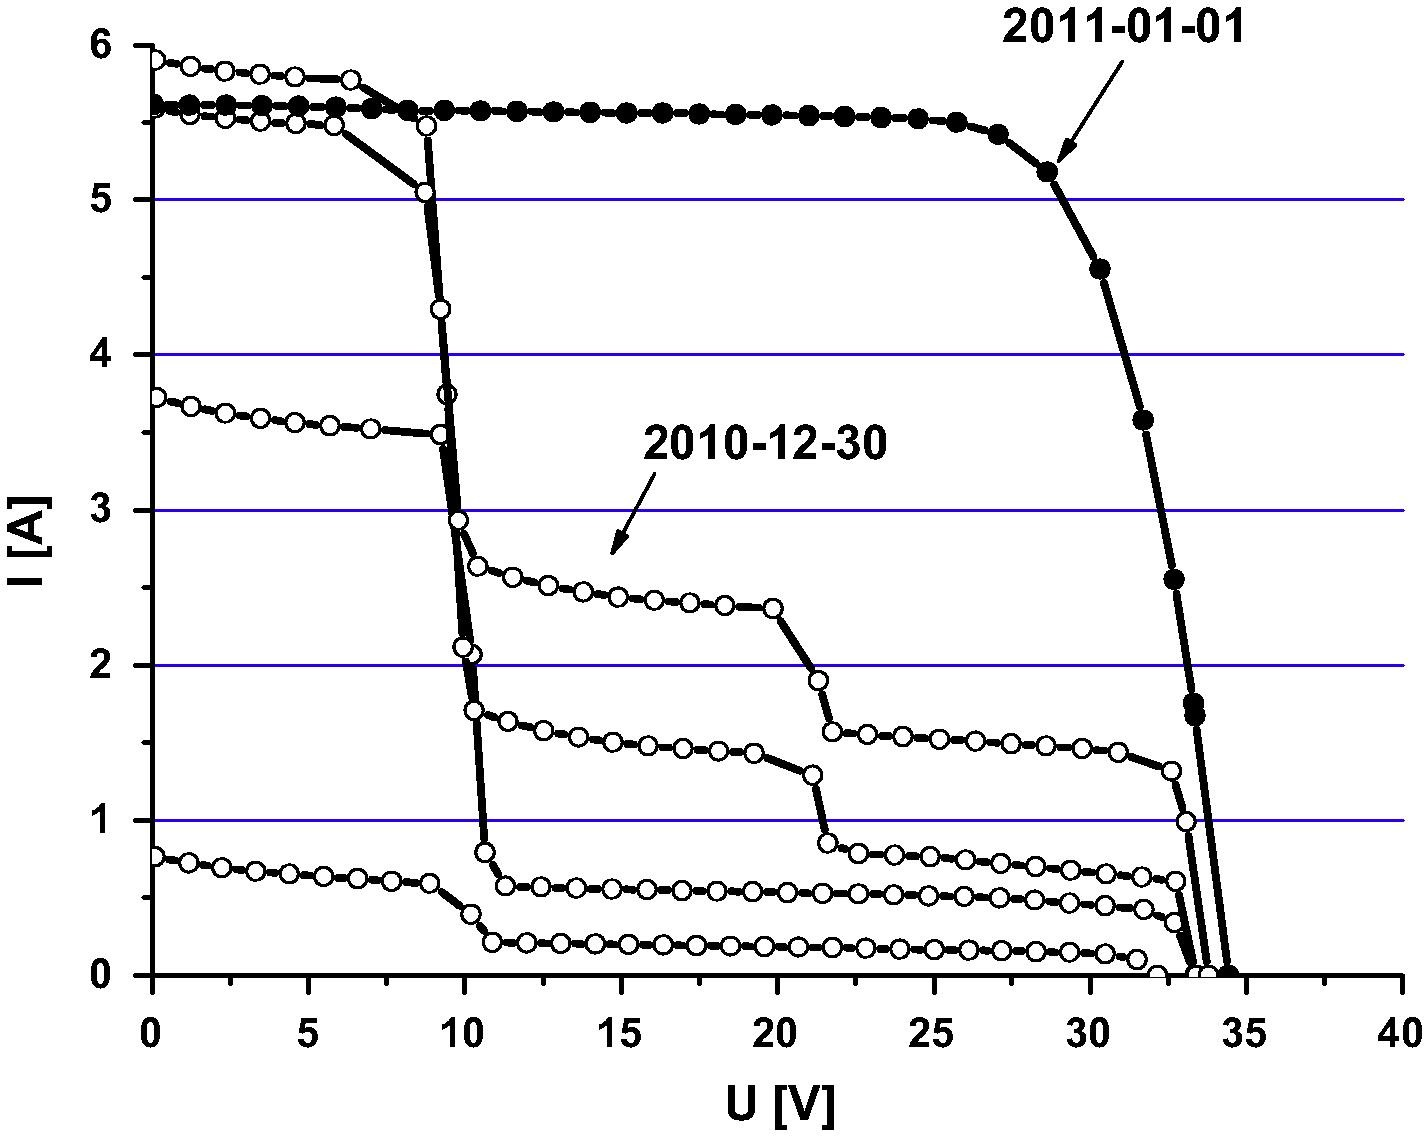
\includegraphics[scale=1.5]{imagens/IxV_schill}
	\caption{Curva característica I-V de painéis fotovoltaicos sobre influência de neve, a qual foi removida no dia 01/01. Fonte: \citeauthorandyear{SCHILL2015259}. }

	\label{fig:CurvaIVNeve}
\end{figure}
\FloatBarrier

Assim como analisado por \citeauthorandyear{martin2017temperature} , a temperatura do painel fotovoltaico possui influência sobre a geração, e respectiva curva I-V do painel em análise. É possível observar esse efeito na Figura~\ref{fig:IVTemp}.

\FloatBarrier
\begin{figure}[!htbp]
	\centering
	%scale redimensiona a figura.
	%1.5 = 150% do tamanho original
	%1 = 100% do tamanho original
	%0.20 = 20% do tamanho original
	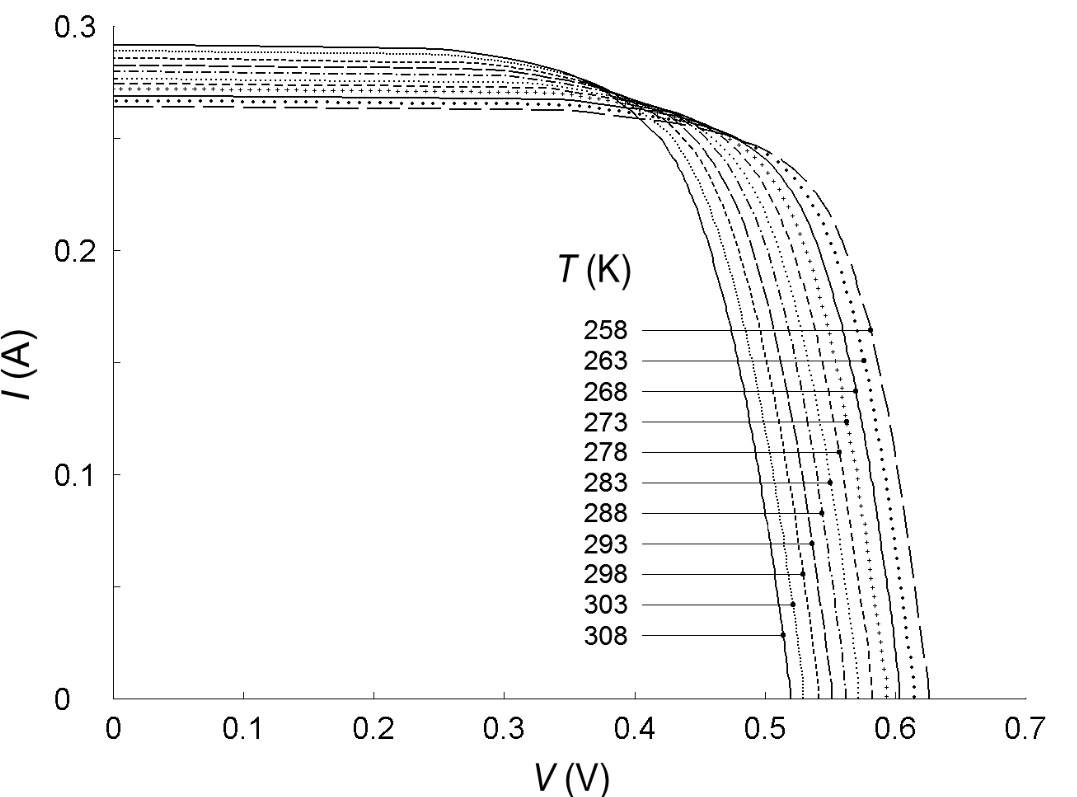
\includegraphics[scale=0.3]{imagens/IxV_Temp}
	\caption{Curva característica I-V de painéis fotovoltaicos sobre diferentes temperaturas. Fonte: \citeauthorandyear{martin2017temperature}. }
	
	\label{fig:IVTemp}
\end{figure}
\FloatBarrier

Assim como aponta \citeauthorandyear{SCHILL2015259}, o elemento central para a geração da curva I-V é a carga eletrônica, o qual tem como principal função simular diferentes cargas para o painel fotovoltaico, de maneira a permitir verificar seu comportamento, como foi descrito também por \citeauthorandyear{aliaga2016experimental}, na criação de sistemas que possam garantir a máxima potência global de um arranjo fotovoltaico. Um sistema de carga eletrônica com MOSFET, como mostrado na figura~\ref{fig:CargaELE} permite a rápida variação de carga sobre o painel fotovoltaico de maneira a possibilitar a construção da curva I-V característica do painel em determinado instante, desta maneira diminuir a diferença de geração devido a meios externos como nuvens ou variações climáticas, \cite{WILLOUGHBY2018171}.%(WILLOUGHBY; OSINOWO, 2018).

\FloatBarrier
\begin{figure}[!htbp]
	\centering
	%scale redimensiona a figura.
	%1.5 = 150% do tamanho original
	%1 = 100% do tamanho original
	%0.20 = 20% do tamanho original
	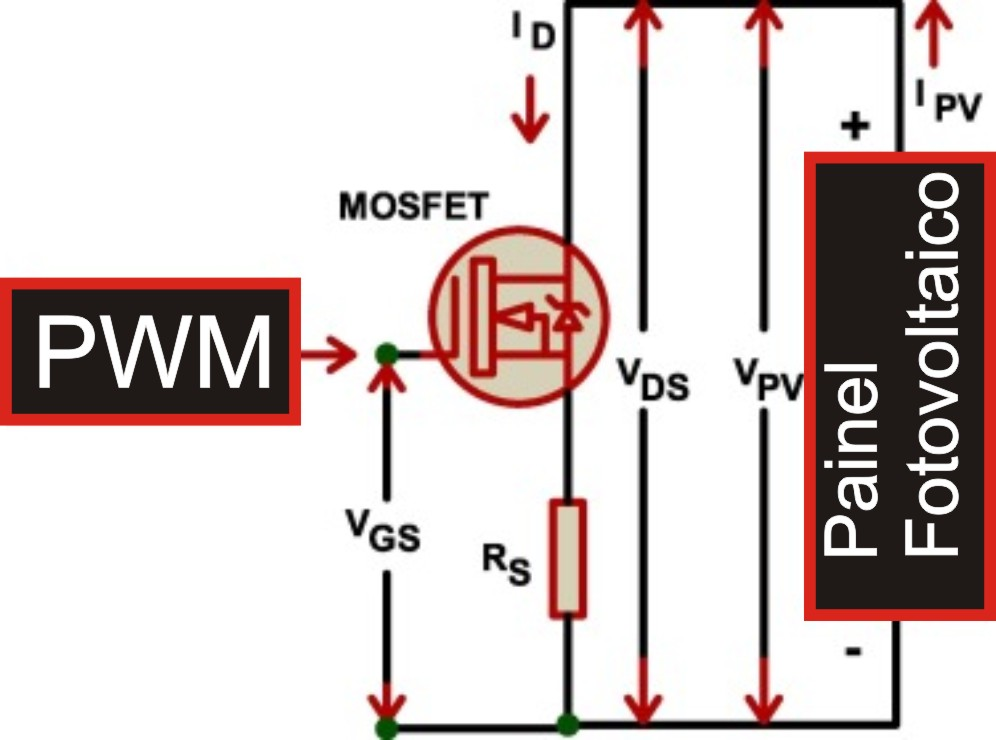
\includegraphics[scale=1]{imagens/MOSFET_LOAD}
	\caption{Uso de MOSFET como carga eletrônica para uso em painéis fotovoltaicos. Fonte: \citeauthorandyear{WILLOUGHBY2018171}. }
	
	\label{fig:CargaELE}
\end{figure}
\FloatBarrier

%\cite




Este é um exemplo de como usar tabelas. Referência cruzada: Tabela~\ref{tab:exemplo}

\FloatBarrier
\begin{table}[!htbp]
\centering
\caption{Exemplo de tabela de 2 colunas}
	\begin{tabular}{ c | c }
		\hline
		\textbf{Coluna 1} & \textbf{Coluna 2} \\ \hline
		Dado 1a           & Dado 1b           \\ \hline
		Dado 2a           & Dado 2b           \\ \hline
		Dado 3a           & Dado 3b           \\ \hline
		Dado 4a           & Dado 4b           \\ \hline
	\end{tabular}
	\\ \vspace{0.2cm}
	\textbf{Fonte:} Elaborada pelo autor
	\label{tab:exemplo}
\end{table}
\FloatBarrier


Este é um exemplo de como usar quadros. Referência cruzada: Quadro~\ref{qua:exemplo}

\FloatBarrier
\begin{quadro}[!htbp]
	\centering
	\caption{Exemplo de quadro}
	\includegraphics[scale=.7]{imagens/exemploQuadro}
	\\\textbf{Fonte:} Elaborada pelo autor
	\label{qua:exemplo}
\end{quadro}
\FloatBarrier


Este é um exemplo de como usar equações. Referência cruzada: Equação~\ref{eq:exemplo}

\begin{equation}
\sum_{i=1}^{n} = \frac{n(n+1)}{2}
\label{eq:exemplo}
\end{equation}


Exemplo de inserção de lista de código fonte (\textbf{\textcolor{red}{não use acentos no código!}}):

\lstinputlisting[language=Java]{fontes/ClasseExemplo.java} 



Este é um exemplo de como inserir texto sem formatação (ambiente verbatim):

\begin{verbatim}
	Texto sem formatação, como espaçamento igual.
\end{verbatim}


Exemplo de lista de itens:

\begin{itemize}
	\item \textbf{Item 1:} texto...;
	\item \textbf{Item 2:} texto...;
    \begin{itemize}
            \item \textbf{Subitem:} texto...;
            \item \textbf{Subitem:} texto...;
            \item \textbf{Subitem:} texto...;
        \end{itemize}
	\item \textbf{Item 3:} texto...;
	\item \textbf{Item n:} texto....
\end{itemize}


Exemplo de lista numerada:

\begin{enumerate}
	\item \textbf{Item:} texto...;
	\item \textbf{Item:} texto...;
    \begin{enumerate}
        \item \textbf{Subitem:} texto...;
        \item \textbf{Subitem:} texto...;
        \item \textbf{Subitem:} texto...;
    \end{enumerate}
	\item \textbf{Item:} texto...;
	\item \textbf{Item:} texto....
\end{enumerate}


Exemplos de comandos para texto e referências:

\begin{itemize}
	\item Para iniciar um novo parágrafo, basta deixar uma linha em branco no código fonte;
	\item Não force o compilador a pular mais de uma linha, pois terá influência negativa na composição do documento;
	\item Sempre deixe o \LaTeX\ realizar a formatação de parágrafos e posicionamento de elementos;
	\item Utilização de aspas simples (abertura \verb|`|, fechamento \verb|'|): `Texto entre aspas simples';
	\item Utilização de aspas duplas (abertura \verb|``|, fechamento \verb|''|): ``Texto entre aspas duplas'';
	\item Negrito (comando \verb|\textbf|): \textbf{texto em negrito};
	\item Itálico (comando \verb|\textit|): \textit{texto em itálico};
	\item Sublinhado (comando \verb|\underline|): \underline{texto sublinhado};
	\item Negrito e itálico (usar comandos juntos): \textbf{\textit{texto em negrito e itálico}};
	\item Alterar cor do texto (comando \verb|\textcolor{cor}{texto}|):
	\begin{itemize}
		\item Exemplo \verb|\textcolor{red}{texto}|: \textcolor{red}{texto vermelho};
		\item Exemplo \verb|\textcolor[RGB]{255, 102, 0}|: \textcolor[RGB]{255, 102, 0}{texto laranja};
		\item Exemplo \verb|\textcolor[HTML]{006AD7}|: \textcolor[HTML]{006AD7}{texto azul};
	\end{itemize}
	\item Ambiente matemático inline (comando \verb|$ expressão $|): $s = x^2-2x +1$;
	\item Referência normal (comando \verb|\cite|):
	\begin{itemize}
		\item \cite{Agaisse1995};
		\item \cite{Abedi2014};
		\item \cite{BtNomenclature2016};
	\end{itemize}
	\item Referência normal com mais de uma obra (comando \verb|\cite|):
	\begin{itemize}
		\item \cite{Agaisse1995, Abedi2014};
		\item \cite{Nelson2014, BtNomenclature2016, AgapitoTenfen2014};
	\end{itemize}
	\item Referência nome e ano (comando \verb|\citeauthorandyear|):
	\begin{itemize}
		\item %\citeauthorandyear{Agaisse1995};
		\item %\citeauthorandyear{Abedi2014};
		\item %\citeauthorandyear{BtNomenclature2016};
	\end{itemize}
\end{itemize}


Exemplo 1 de referência direta:

\begin{citacao}
	Os 20 aminoácidos usualmente encontrados como resíduos em proteínas contém um grupo $\alpha$-carboxil, um grupo $\alpha$-amino e um grupo R distinto substituído no átomo de carbono $\alpha$. O átomo de carbono $\alpha$ de todos os aminoácidos, com exceção da glicina, é assimétrico e, portanto, os aminoácidos podem existir em pelo menos duas formas estereoisoméricas. Somente os estereoisômeros L, com uma configuração relacionada à configuração absoluta da molécula de referência L-gliceraldeído, são encontrados em proteínas \cite[p. 81]{Nelson2014}
\end{citacao}

Exemplo 2 de referência direta:

\begin{citacao}
	\textit{These various insecticidal proteins are synthesized during the stationary phase and accumulate in the mother cell as a crystal inclusion which can account for up to 25\% of the dry weight of the sporulated cells. The amount of crystal protein produced by a B. thuringiensis culture in laboratory conditions (about 0.5 mg of protein per ml) and the size of the crystals (24) indicate that each cell has to synthesize $10^6$ to $2 \times 10^6$ $\delta$-endotoxin molecules during the stationary phase to form a crystal} \cite[p. 1]{Agaisse1995}
\end{citacao}

Exemplo de nota de rodapé\footnote{Essa é uma nota de rodapé!}.
